\subsection{Diagrammatic temporal conversion rendering}\label{app:feynman-dict}
\paragraph{Diagrammatic rendering.} The collision/export rows may also be rendered in a diagrammatic dictionary view after the cited row has been fixed. The rendering below is a later compression of the same integer ledgers recorded for Example~E6 in the cited Supplement A row set.

\begin{center}
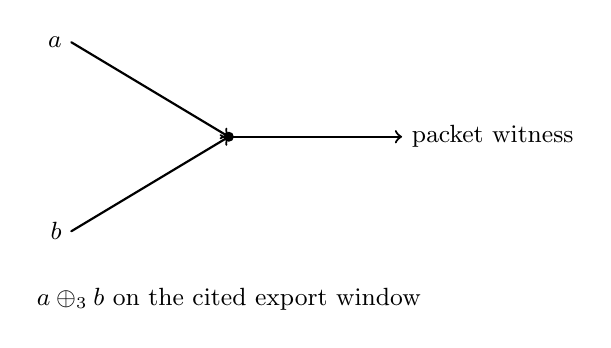
\begin{tikzpicture}[x=1cm,y=1cm, line cap=round, line join=round, every node/.style={font=\small}]
  % vertex
  \filldraw[black] (0,0) circle (1.6pt);
  % incoming/outgoing legs
  \draw[thick,->] (-2,1.2) -- (0,0);
  \draw[thick,->] (-2,-1.2) -- (0,0);
  \draw[thick,->] (0,0) -- (2.2,0);
  \node[left] at (-2,1.2) {$a$};
  \node[left] at (-2,-1.2) {$b$};
  \node[right] at (2.2,0) {packet witness};
  \node[below] at (0,-1.8) {$a\oplus_3 b$ on the cited export window};
\end{tikzpicture}
\end{center}

\paragraph{Anchor.} Use this rendering only with an explicit citation to the corresponding cited collision/export row and its cut residual check.
